
\section{Μη οπτική μεταγωγή}

Όπως αναφέρθηκε, η ηλεκτρική μεταγωγή κυριαρχεί το μεγαλύτερο μέρος
των οπτικών επικοινωνιών. Αν και αυτό απαιτεί την μετατροπή του
οπτικού σήματος σε ηλεκτρικό και μετά ξανά πίσω στο οπτικό, οι
ταχύτητες όπου είναι δυνατόν να επιτευχθούν είναι της τάξης των
400Gbps \cite{8207825}. Επίσης πολλαπλά τέτοια σήματα μπορούν να
πολυπλεχτούν και να περάσουν από μία μοναδική ίνα προσφέροντας
πολλαπλάσια ταχύτητα όπου φτάνει στα 1.6Tbps.

Κάποιες λύσεις βασίζονται αποκλειστικά στην στην πολυπλεξία μήκους
κύματος (WDM) πολλαπλών ποιο αργών σημάτων ταχύτητας 50, 25 ή 10Gbps
\cite{8438591}\cite{7526271}\cite{1700008}, όπου η χρήση συμβατικών
switches είναι εφικτή. Ο τρόπος με τον οποίος μπορεί να επιτευχθεί
αυτό είναι απλός, διότι η προτυποποιημένη υποδοχή SFP όπου έχουν τα
περισσότερα επαγγελματικά switches επιτρέπει την μετατροπή ηλεκτρικού
ethernet σήματος σε διάφορα άλλα (όπως οπτικό). Η μετατροπή του
ηλεκτρικού σήματος σε οπτικό και αντίστοιχα του οπτικού σε ηλεκτρικό
γίνεται πάνω στον SFP αντάπτορα οπότε η χρήση διαφορετικών μηκών
κύματος γίνεται με την εισαγωγή του κατάλληλου αντάπτορα. Τα πολλαπλά
αυτά οπτικά σήματα τα οποία μεταδίδονται σε ξεχωριστές ίνες,
πολυπλέκονται σε έναν WDM πολυπλέκτη ο οποίος συνενώνει τα διάφορα
σήματα και τα μεταδίδει μέσω μίας οπτικής ίνας. Εκεί που καταλήγει η
οπτική ίνα, αντιστρέφεται η διαδικασία με την χρήση αντίστοιχου
εξοπλισμού.

\begin{figure}[h]
  \centering
  \begin{subfigure}{0.4\linewidth}
    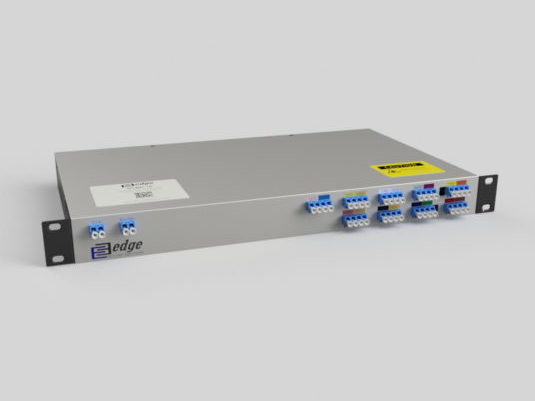
\includegraphics[width=\textwidth]{wdm.jpg}
    \caption{DCMD-18}
    \label{wdm}
  \end{subfigure}
~
  \begin{subfigure}{0.4\linewidth}
    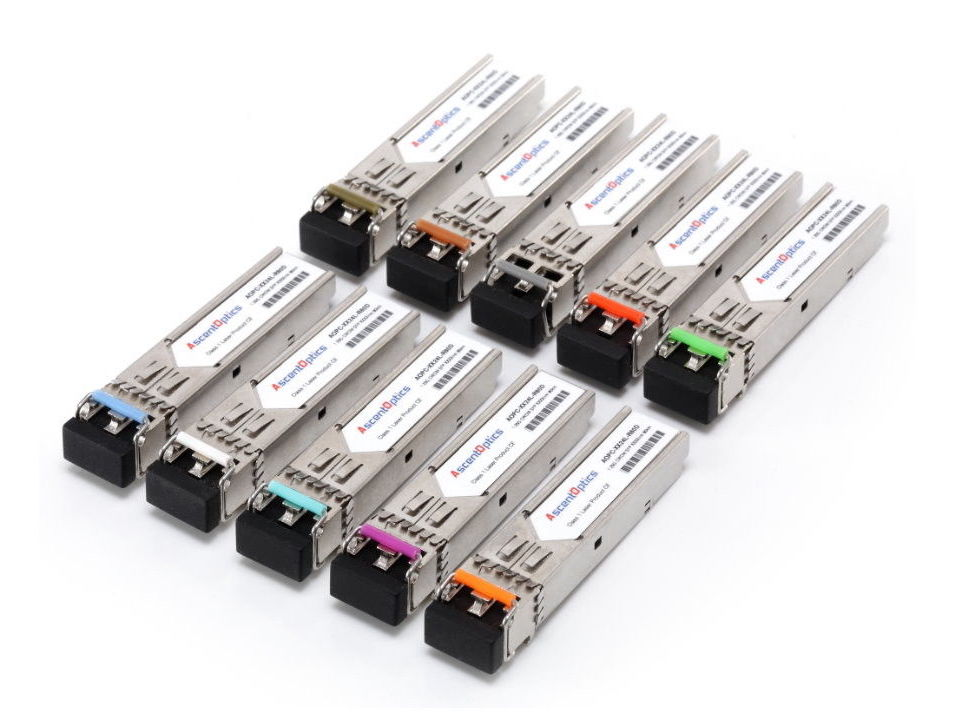
\includegraphics[width=\textwidth]{sfp.jpg}
    \caption{SFP modules}
    \label{sfp}
  \end{subfigure}
  \caption{(\ref{wdm}) 18 Channels Double Fiber Passive CWDM Mux/Demux by
    edge optical solutions (\ref{sfp}) SFP modules for different wave lengths
    by Accent Optics}
\end{figure}

%%% Local Variables:
%%% mode: latex
%%% TeX-master: "main"
%%% End:
